\section{Motivation and Observation}
\label{sec:observation}

\begin{figure}
	\centering
	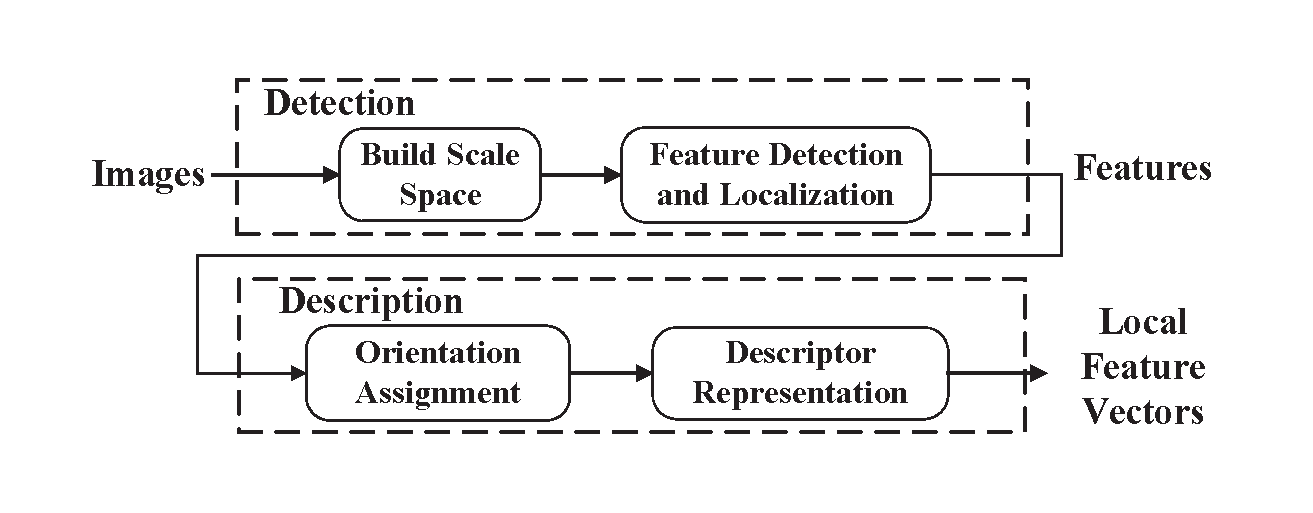
\includegraphics[width=3.5in]{images/fig-workflow.eps}
	\caption{Process flow of a typical local feature descriptor.}
	\label{fig:workflow}
\end{figure}

\begin{figure*}[!t]
	\centering
	\subfigure[Salient region has the densest local features.]{
		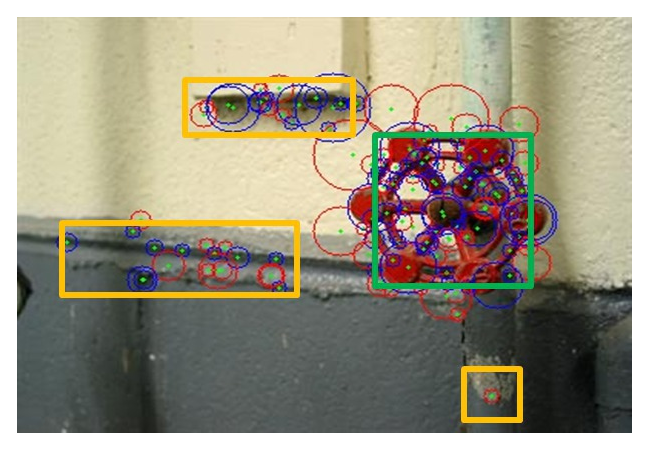
\includegraphics[width=2.5in]{images/fig-observation1.eps}
		\label{fig:observation_1}
	}
	\hfil
	\subfigure[Several salient regions in one image.]{
		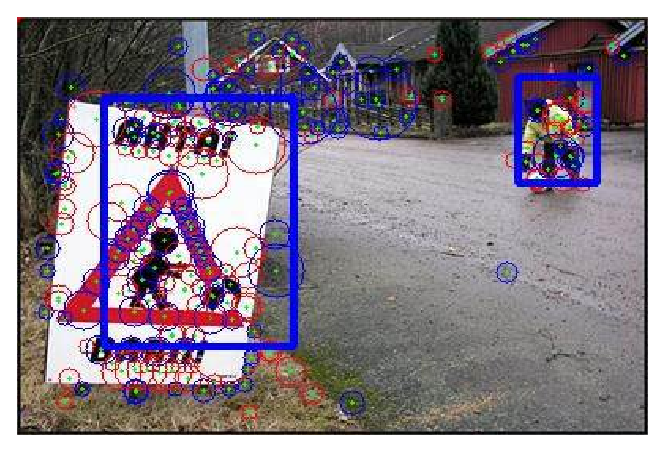
\includegraphics[width=2.5in]{images/fig-observation2.eps}
		\label{fig:observation_2}
	}
	\caption{Example images with local feature based salient regions}
	\label{fig:observations}
\end{figure*}

\subsection{Motivation}

Due to their high accuracy, local feature-based algorithms have been widely used in real-world applications.  As shown in Figure~\ref{fig:workflow}, they generally consist of two stages: detection stage and description stage.  An overview of their processing workflow is shown as follows:

\begin{itemize}
\setlength{\itemsep}{0mm}


\item \textbf{Feature Detection Stage:} This stage is to detect \emph{feature points} in an image or a video frame. After an image is loaded and initialized, a \emph{m*n} scale space pyramid is constructed to guarantee scale invariant.  After building the scale pyramid, each point in the pyramid is compared with its
surrounding 26 points in a 3*3*3 cubic. If its value is the extreme value~(maximum or minimum), the point is chosen as a feature point candidate. To guarantee the quality of extracted points, the candidate points with low contrast or localized along edges will be discarded. The remaining points are the final feature points.

\item \textbf{Feature Description Stage:} In this stage, each detected point will be described by a high-dimensional vector. First, to make the algorithm rotation invariant, a orientation value is calculated based on the information around it . Then, a descriptor window is constructed and the vector is computed based on the orientation information. The vector value is also normalized to keep the algorithm illumination invariant.
\end{itemize}


There exist two major issues for these local feature descriptors. First, the processing speed of these local feature descriptors are very slow and among their two stages, description stage is more time-consuming. Therefore, the description stage is more time-consuming than the detection stage. Second, since these algorithms use a multi-dimensionality vector to represent a feature point, the space requirement is also high to storage the feature points for an image or a video frame. To illustrate these two problems, we evaluate the processing time, space requirement, the point number and the proportion between two stages based on two most widely used algorithms SIFT and SURF. The hardware is a I7 CPU with 4G memory. The dataset is that used in ~\cite{mikolajczyk2005performance}. As the data shown in Table \ref{tab:surfandsift}, it can only finish less than five image processing on a I7 machine and the processing time of description stage is at least twice compared to that of the detection stage. Moreover, there are about one thousand points in each image averagely and each image requires about several KB space to storage its feature points.

\begin{table}[!t]
\begin{center}
\begin{tabular}{|l|c|c|c|c|}
\hline
 & Time(ms) & Space(KB) & Pnum & Proportion \\
\hline
SURF & 171 & 269 & 989   &  1:2\\\hline
SIFT & 719 & 1437 & 2723 & 1:3 \\\hline
\end{tabular}
\end{center}
\caption{Typical time and space consumption of local feature descriptor.}
\label{tab:surfandsift}
\end{table}

As the data shown, no matter the processing time or the storage space is proportional to the amount of feature points in an image. Therefore, less feature points means  less processing time and less storage space. Salient region techniques, which picks up the visual attention parts from an image, can be used to reduced the amount of feature points through marking the features outside the region as unimportant and eliminating them. Although there have existed many mature salient region algorithms~\cite{cheng2011global,achanta2009frequency,itti1998model}, they are not designed to work with local features. However, prior salient region detection algorithms are independent on the process of local feature-based algorithms. Therefore,  combining them would involve additional overhead, which may degrade the final performance.

\subsection{Observation}
\label{subsec:observation}

To overcome these obstacles, we make a comprehensive analysis on the relation between the salient region and the distribution of feature points  in images. After studying carefully on the distribution of feature points, we get three major observations:



\begin{description}
	
\item[Observation 1] \desclabel{itm:observation_1} \textit{A salient region has more dense local features.} It means local features in the salient region are closer to each other, while noise features or unimportant features are far away from them. As shown in Figure \ref{fig:observation_1}, local features in the salient region (green box) gather together and many obviously noises locate far away from that box. 

\item[Observation 2] \desclabel{itm:observation_2} \textit{The region with dense  local features is the preferred salient region.} Also from Figure \ref{fig:observation_1}, the density of feature points in green box is larger compared to that of points in the other two yellow boxes. 

\item[Observation 3] \desclabel{itm:observation_3} \textit{There may exist several salient regions in an image.} In other words, there exists several clusters of local features in an image. For example, the photo in Figure \ref{fig:observation_2} contains two objects, a person and a stop sign, which shape two salient regions following two clusters of local features.

\end{description}

Observation~\ref{itm:observation_1} and \ref{itm:observation_2} indicate a possibility that we can compute the salient region directly based on the distribution of local features, which means salient regions can be performed just after the detecting stage of local feature descriptor. In addition, Observation~\ref{itm:observation_3} means it's necessary to deal with multiple distribution of feature points should be computed for multiple salient regions. Based on these observations, it is possible to compute the salient region based on the information of local feature-based descriptors, which can be used to further optimize the processing speed and storage requirement of local feature-based descriptors.